% Options for packages loaded elsewhere
\PassOptionsToPackage{unicode}{hyperref}
\PassOptionsToPackage{hyphens}{url}
%
\documentclass[
]{article}
\usepackage{amsmath,amssymb}
\usepackage{lmodern}
\usepackage{iftex}
\ifPDFTeX
  \usepackage[T1]{fontenc}
  \usepackage[utf8]{inputenc}
  \usepackage{textcomp} % provide euro and other symbols
\else % if luatex or xetex
  \usepackage{unicode-math}
  \defaultfontfeatures{Scale=MatchLowercase}
  \defaultfontfeatures[\rmfamily]{Ligatures=TeX,Scale=1}
\fi
% Use upquote if available, for straight quotes in verbatim environments
\IfFileExists{upquote.sty}{\usepackage{upquote}}{}
\IfFileExists{microtype.sty}{% use microtype if available
  \usepackage[]{microtype}
  \UseMicrotypeSet[protrusion]{basicmath} % disable protrusion for tt fonts
}{}
\makeatletter
\@ifundefined{KOMAClassName}{% if non-KOMA class
  \IfFileExists{parskip.sty}{%
    \usepackage{parskip}
  }{% else
    \setlength{\parindent}{0pt}
    \setlength{\parskip}{6pt plus 2pt minus 1pt}}
}{% if KOMA class
  \KOMAoptions{parskip=half}}
\makeatother
\usepackage{xcolor}
\IfFileExists{xurl.sty}{\usepackage{xurl}}{} % add URL line breaks if available
\IfFileExists{bookmark.sty}{\usepackage{bookmark}}{\usepackage{hyperref}}
\hypersetup{
  pdftitle={Alcohol and Asteroids},
  pdfauthor={Jon Mellon},
  hidelinks,
  pdfcreator={LaTeX via pandoc}}
\urlstyle{same} % disable monospaced font for URLs
\usepackage[margin=1in]{geometry}
\usepackage{color}
\usepackage{fancyvrb}
\newcommand{\VerbBar}{|}
\newcommand{\VERB}{\Verb[commandchars=\\\{\}]}
\DefineVerbatimEnvironment{Highlighting}{Verbatim}{commandchars=\\\{\}}
% Add ',fontsize=\small' for more characters per line
\usepackage{framed}
\definecolor{shadecolor}{RGB}{248,248,248}
\newenvironment{Shaded}{\begin{snugshade}}{\end{snugshade}}
\newcommand{\AlertTok}[1]{\textcolor[rgb]{0.94,0.16,0.16}{#1}}
\newcommand{\AnnotationTok}[1]{\textcolor[rgb]{0.56,0.35,0.01}{\textbf{\textit{#1}}}}
\newcommand{\AttributeTok}[1]{\textcolor[rgb]{0.77,0.63,0.00}{#1}}
\newcommand{\BaseNTok}[1]{\textcolor[rgb]{0.00,0.00,0.81}{#1}}
\newcommand{\BuiltInTok}[1]{#1}
\newcommand{\CharTok}[1]{\textcolor[rgb]{0.31,0.60,0.02}{#1}}
\newcommand{\CommentTok}[1]{\textcolor[rgb]{0.56,0.35,0.01}{\textit{#1}}}
\newcommand{\CommentVarTok}[1]{\textcolor[rgb]{0.56,0.35,0.01}{\textbf{\textit{#1}}}}
\newcommand{\ConstantTok}[1]{\textcolor[rgb]{0.00,0.00,0.00}{#1}}
\newcommand{\ControlFlowTok}[1]{\textcolor[rgb]{0.13,0.29,0.53}{\textbf{#1}}}
\newcommand{\DataTypeTok}[1]{\textcolor[rgb]{0.13,0.29,0.53}{#1}}
\newcommand{\DecValTok}[1]{\textcolor[rgb]{0.00,0.00,0.81}{#1}}
\newcommand{\DocumentationTok}[1]{\textcolor[rgb]{0.56,0.35,0.01}{\textbf{\textit{#1}}}}
\newcommand{\ErrorTok}[1]{\textcolor[rgb]{0.64,0.00,0.00}{\textbf{#1}}}
\newcommand{\ExtensionTok}[1]{#1}
\newcommand{\FloatTok}[1]{\textcolor[rgb]{0.00,0.00,0.81}{#1}}
\newcommand{\FunctionTok}[1]{\textcolor[rgb]{0.00,0.00,0.00}{#1}}
\newcommand{\ImportTok}[1]{#1}
\newcommand{\InformationTok}[1]{\textcolor[rgb]{0.56,0.35,0.01}{\textbf{\textit{#1}}}}
\newcommand{\KeywordTok}[1]{\textcolor[rgb]{0.13,0.29,0.53}{\textbf{#1}}}
\newcommand{\NormalTok}[1]{#1}
\newcommand{\OperatorTok}[1]{\textcolor[rgb]{0.81,0.36,0.00}{\textbf{#1}}}
\newcommand{\OtherTok}[1]{\textcolor[rgb]{0.56,0.35,0.01}{#1}}
\newcommand{\PreprocessorTok}[1]{\textcolor[rgb]{0.56,0.35,0.01}{\textit{#1}}}
\newcommand{\RegionMarkerTok}[1]{#1}
\newcommand{\SpecialCharTok}[1]{\textcolor[rgb]{0.00,0.00,0.00}{#1}}
\newcommand{\SpecialStringTok}[1]{\textcolor[rgb]{0.31,0.60,0.02}{#1}}
\newcommand{\StringTok}[1]{\textcolor[rgb]{0.31,0.60,0.02}{#1}}
\newcommand{\VariableTok}[1]{\textcolor[rgb]{0.00,0.00,0.00}{#1}}
\newcommand{\VerbatimStringTok}[1]{\textcolor[rgb]{0.31,0.60,0.02}{#1}}
\newcommand{\WarningTok}[1]{\textcolor[rgb]{0.56,0.35,0.01}{\textbf{\textit{#1}}}}
\usepackage{longtable,booktabs,array}
\usepackage{calc} % for calculating minipage widths
% Correct order of tables after \paragraph or \subparagraph
\usepackage{etoolbox}
\makeatletter
\patchcmd\longtable{\par}{\if@noskipsec\mbox{}\fi\par}{}{}
\makeatother
% Allow footnotes in longtable head/foot
\IfFileExists{footnotehyper.sty}{\usepackage{footnotehyper}}{\usepackage{footnote}}
\makesavenoteenv{longtable}
\usepackage{graphicx}
\makeatletter
\def\maxwidth{\ifdim\Gin@nat@width>\linewidth\linewidth\else\Gin@nat@width\fi}
\def\maxheight{\ifdim\Gin@nat@height>\textheight\textheight\else\Gin@nat@height\fi}
\makeatother
% Scale images if necessary, so that they will not overflow the page
% margins by default, and it is still possible to overwrite the defaults
% using explicit options in \includegraphics[width, height, ...]{}
\setkeys{Gin}{width=\maxwidth,height=\maxheight,keepaspectratio}
% Set default figure placement to htbp
\makeatletter
\def\fps@figure{htbp}
\makeatother
\setlength{\emergencystretch}{3em} % prevent overfull lines
\providecommand{\tightlist}{%
  \setlength{\itemsep}{0pt}\setlength{\parskip}{0pt}}
\setcounter{secnumdepth}{5}
\ifLuaTeX
  \usepackage{selnolig}  % disable illegal ligatures
\fi

\title{Alcohol and Asteroids}
\author{Jon Mellon}
\date{2022-03-07}

\begin{document}
\maketitle

Like every social scientist who has had to think about pregnancy for the first time, I quickly came across Emily Oster's book: \href{https://www.goodreads.com/book/show/16158576-expecting-better?from_search=true\&from_srp=true\&qid=5FmElbF5mM\&rank=1}{Expecting Better: Why the Conventional Pregnancy Wisdom is Wrong---and What You Really Need to Know}. Oster proposes using decision theory to use data on different activities during pregnancy to make decisions that best reflect your preferences.

The most controversial aspect of the book has been her claim that there is no risk to light drinking during pregnancy. This view has been criticized quite intensely, but I think these critiques don't get to the heart of the issue.\footnote{I'll talk through some of my issues with those studies in a future post.} While I don't think the evidence is decisive either way on light drinking and pregnancy, Oster's analysis implicitly builds in some strong statistical assumptions that readers should carefully consider before they accept her conclusions.

Oster starts by saying:

\begin{quote}
One phrase I kept coming across was ``no amount of alcohol has been proven safe.'' The implication, I suppose, is that we know that there exists a level of drinking that is bad, so we should assume all other levels are bad until proven otherwise.
\end{quote}

I think that is a slightly unfair read of what the conventional wisdom is saying. I think a charitable reading of the conventional wisdom is as follows: ``We know that there is a level of drinking that is bad and that at some point (probably before literally zero drinking) its effect falls very close to zero''.

This view implies a prior that looks something like the following:\footnote{The distribution is simulated as follow in R: c(rep(0,10000), -rexp(10000) * 2, rexp(100)/5). 49.8\% of the prior probability mass is on an effect of exactly zero, 49.8\% spread over an exponential distribution in the negative direction and 0.5\% spread over a positive exponential distribution.}

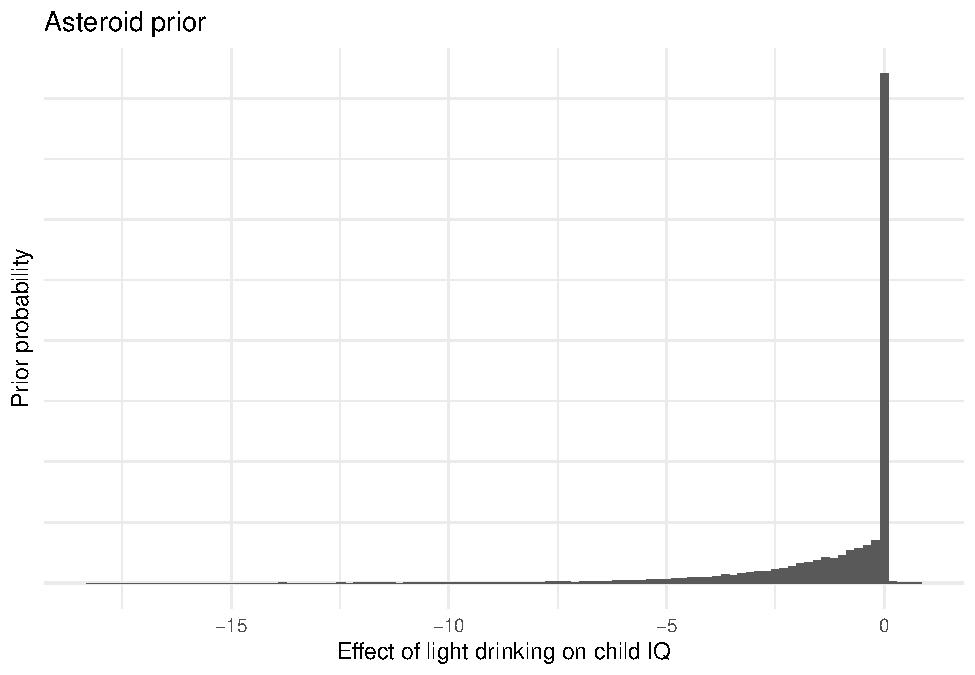
\includegraphics{index_files/figure-latex/unnamed-chunk-1-1.pdf}

There's a large point mass at exactly zero, but a non-zero probability that the effect is actually negative. Crucially, this view gives zero (or trivially low) credence to the idea that light drinking might boost child IQ.

I'm going to refer to this colloquially as the asteroid prior. The effect of an asteroid is usually exactly zero (because it misses the earth or burns up in the atmosphere), but if it does get through, the outcomes are all some version of bad.\footnote{If you want to add on a small tail of positive outcomes to the prior that's fine too (perhaps the asteroid hits Vladmir Putin and ends the invasion of Ukraine), but for the levels of evidence we're talking about it's not going to matter.} In this analogy, the scientific question is just whether alcohol makes it through to cause harm, no one disagrees about the direction of the effect if it does.

You might think that holding an asteroid prior such as this is unscientific and that no quality of evidence could ever convince someone who holds it. While it is true that this prior will always say that light drinking is bad in expectation, high quality evidence could hypothetically reduce the plausible effect size to very close to zero and make the probability that the effect size is exactly zero arbitrarily high. If the evidence suggested that there is a 99\% chance that the effect is exactly zero and that---if it is non-zero---there is a 99\% chance that the effect has a smaller magnitude than 0.2 IQ points, few people would think it was worth advising against light drinking.

My read of Oster is that she is implicitly interpreting all the studies using a symmetric prior (e.g.~the one below) around zero.\footnote{It's worth noting that the actual studies under discussion all use frequentist methods. The Bayesian language here is a way of conceptualizing how a reader could reasonably update their views based on reading the studies. You certainly could formalize this into a Bayesian meta-analysis, but the concepts from Bayesian statistics are helpful even when doing this informally. Note that if you were to do this formally, you would want to include latent estimates of measurement error at the study level as part of the estimation.} This is a very standard assumption in social science studies, as we rarely have strong enough theories to convincingly rule out effects in a particular direction. There are good arguments for minimum wages increasing employment or for decreasing it. If you ran a minimum wage study with a heavily asymmetric prior, you would rightly be called out for stacking the deck.

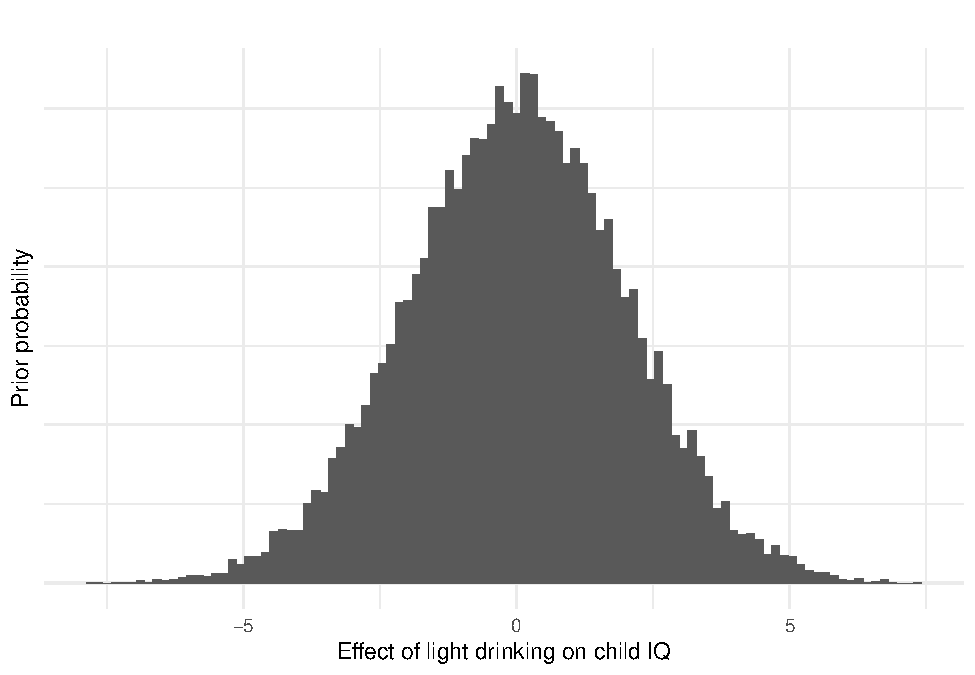
\includegraphics{index_files/figure-latex/unnamed-chunk-2-1.pdf}

So which prior should we be using when assessing the alcohol and pregnancy literature. I'm not a biologist, but the asteroid prior seems to fit quite well with Oster's own account of the mechanisms:

\begin{quote}
When you drink\ldots{} Your liver processes the alcohol into a chemical called acetaldehyde and then into acetate. The acetaldehyde is toxic to other cells, and depending on how quickly you drink, it can remain in your bloodstream. You share your blood with your baby through the placenta; acetaldehyde, which remains in your bloodstream, is therefore shared with the fetus\ldots{}\textbf{If too much acetaldehyde is passed to the baby, it can get into his tissues and impact development. When you drink slowly, you metabolize much of the alcohol before it would get to the fetus. If you drink quickly, your liver cannot keep up and toxins are passed to the fetus.}
\end{quote}

The story here is that alcohol is bad, but the mother's body is probably capable of dealing with the negative effects of it before it reaches the fetus. Notably, there's no counterbalancing story here about perhaps acetaldehyde having some positive effects in the right dose. The story also doesn't a priori rule out an effect of light drinking. Instead, the effect is dependent on the empirical facts about how fast and effectively the liver can remove the toxins, the concentration of acetaldehyde required to cause tissue damage etc. The story also doesn't rule out the possibility that some subset of women's bodies will fail to remove the toxins fast enough to avoid damage (maybe depending on ethnicity or body mass?).

So what does the evidence Oster cites say? Is it strong enough to at least shift the asteroid posterior to a large point mass at zero and a small effect otherwise? I'm not aiming to do a literature review of the pregnancy and alcohol literature here, but having read the studies Oster approvingly cites, I'm not convinced that the evidence is strong enough to make us strongly update our posterior.

There are some studies showing negative effects of light alcohol consumption on development, but Oster is skeptical about the quality of these studies. I generally agree with her assessment and agree that the studies she prefers are stronger.\footnote{Since I haven't done a full review of the literature I can't independently say whether the studies she highlights on each side are representative of the literature or whether newer studies show the same results.} Oster's preferred studies are a large Australian prospective cohort study and a similar study on women in England. Not only do these studies not find a negative effect of drinking on IQ:

\begin{quote}
many of these studies actually find that women who drink moderately in pregnancy have children with higher IQ scores
\end{quote}

A positive effect of drinking on IQ sounds like good news for Oster's case. If you have a prior that is symmetrical around zero, the Australian study may represent some modest evidence about light drinking being safe or maybe even slightly beneficial.

However, if you have an asteroid prior, you probably don't believe the positive effect and instead see it as evidence that the study is confounded. This seems to be the view of the researchers:

\begin{quote}
Most researchers agree this effect is probably not causal, and may be due to the fact that women who drink moderately, at least outside of the United States, tend to be better educated than those who do not.
\end{quote}

But is a positive effect at least evidence in favor of exactly zero effect size? What if the confounder is sufficient to actually reverse the effect direction? Oster addresses this concern by saying:

\begin{quote}
The English study I mentioned above is a good antidote to this concern: the authors are able to use the drinking behavior of fathers to adjust for these baseline differences. And, reassuringly, they find no effect of light drinking on IQ.
\end{quote}

This interpretation of null results after adjusting for confounders is ubiquitous in social science, but it's probably incorrect.

If we look at that \href{https://www.nature.com/articles/pr2008261/tables/4}{study}, we see that the authors initially find positive effects of drinking on IQ and that this effect gradually decreases to zero after they load the model up with a huge number of sociodemographic controls.

In fact, they only get the effect size to zero once they control for unmeasured confounders using father's behavior as a proxy. The large drop in effect size when controlling for father's behavior should be a big warning sign. The fact that the father controls change the results, shows that the father proxy is capturing something important that is not captured in the other control variables.

But whatever the father effect is capturing, it is presumably only an imperfect proxy for the true causal variables. This actually means that our best guess about what the effect would be if we fully controlled for what the father effects are proxying for should be a negative effect on IQ (although there could be other countervailing effects we have missed).

Here's a quick simulation to show this intuition. I'm simulating the following causal graphs where each of the arrows is causal probabilistically.

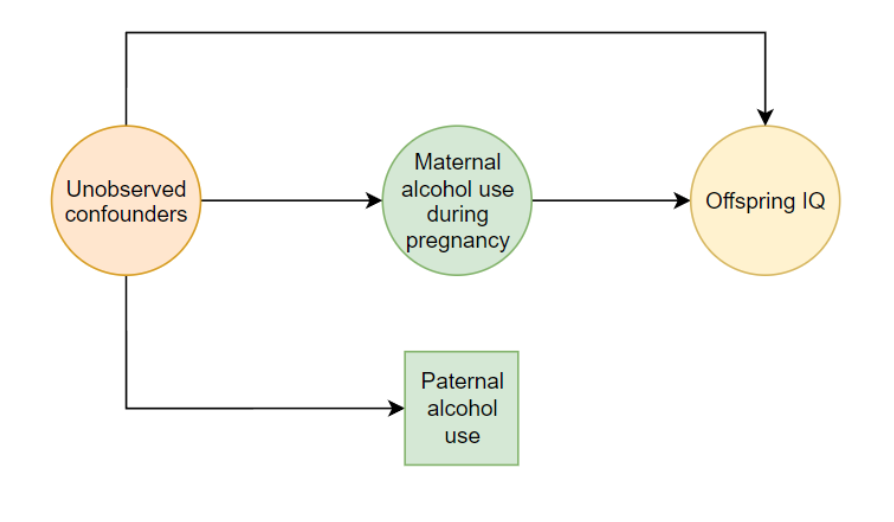
\includegraphics{"/index_files/figure-html/dagalcohol.png"}

\begin{Shaded}
\begin{Highlighting}[]
\FunctionTok{getwd}\NormalTok{()}
\end{Highlighting}
\end{Shaded}

\begin{verbatim}
## [1] "C:/Users/Jon/Documents/stats_blog/drafts/oster_pregnancy_alcohol"
\end{verbatim}

\end{document}
